\chapter{数学导论 - 线性代数基础:矩阵}


\begin{figure}[ht]
  \centering
  \includegraphics[width=1\textwidth]{asset/茶桁的 AI 秘籍_Math_3.png}
\end{figure}

\newpage

上节课我带大家回顾了一下函数和导数的相关概念, 微积分的部分并未结束, 后面还有很多详细的相关内容. 但是在基础课中, 暂时先学这么多. 

这节课来回顾一下线性代数的基础. 

\hypertarget{3.线性代数基础}{}
\section{矩阵}

线性代数, 我们在基础课里主要是讲矩阵相关的东西. 

大家肯定都听过矩阵, 我们经常会听到 \textit{对矩阵做什么运算, 克拉莫法则、Jacobian matrix} 之类的. 但是为什么需要矩阵呢?

先看下面这个公式, 矩阵的形式就是这样子:

\begin{align*}
  \begin{bmatrix}
    a_{11} & a_{12} & \cdots & a_{1n} \\
    a_{21} & a_{22} & \cdots & a_{2n} \\
    \vdots & \vdots & \vdots & \vdots \\
    a_{m1} & a_{m2} & \cdots & a_{mn}
  \end{bmatrix}
\end{align*}

我现在就给大家介绍一下, 矩阵其实就是一些量的排列, 它分行和列. 比如说上面的公式中, 每个数都有一个下标, 我们先来只观察下标. 下标里的数字, 前面的数字代表了是第几行, 后面一个数字代表是第几列. 

比如第一行中, $a_{11}, a_{12}$一直到$a_{1n}$, $a_{1n}$代表这个数它是第 1 行的第 n 列, 同样$a_{m1}$是第 m 行第 1 列, 这就是矩阵的表示. 

\section{鸡兔同笼}

有一个问题, 是古代的一部数学著作《\textit{孙子算经}》里面的一个问题:

\begin{quotation}
  \textit{今有雉兔同笼, 上有三十五头, 下有九十四足, 问雉兔各几何? - 孙子算经}
\end{quotation}

就是问我们鸡兔同笼的问题, 大家应该或多或少都听过. 鸡和兔加在一起 35 只, 它们的脚加在一起 94 只, 问鸡和兔各有多少个?这个问题我相信大家可能在小学就有学过. 那我们来用一个比较常规点的办法去想一下这个东西要怎么去做:

解: 设笼中有小鸡$x$只, 兔子$y$只

\begin{align*}
  & \begin{split} \begin{cases} x + y = 35 & ...(1) \\ 2x + 4y = 94 & ...(2) \end{cases}  \end{split} \\
  & (2)-(1)\times 2\mbox{得:}\\
  & \begin{split} \begin{cases} x+y=35 & ...(3) \\ 2y=24  & ...(4) \end{cases} \end{split} \\
	& (4)\div 2 \mbox{得:} \\
	& \begin{split} \begin{cases} x+y=35 & ...(5) \\ y=12 & ...(6) \end{cases} \end{split} \\
	& (5)-(6) \mbox{得:} \\
	& \begin{split} \begin{cases} x=23 & ...(7) \\ y=12 & ...(8) \end{cases} \end{split}
\end{align*}

首先我们设这个笼中呢有小鸡$x$只,兔子$y$只. 然后建立一个二元一次方程组. 

先是$x+y=35$, 加一块 35 只, 然后$2x+4y=94$, 有 94 只脚. 按照如上步骤, 第二个式子减去(1)式乘 2, 我们再把(4)式除 2, 然后 y 就解出来了, 最后再(5)式减去(6)式, 我们就把$x$也给求出来了. 所以最终答案呢就是 23 只鸡, 12 只兔子. 

\section{线性方程组}

以上方程组很常规对吧?在这里再问大家一个问题: 你们觉得线性方程组与线性方程组之间是由什么导致了不同, 最终唯一确定的?

\begin{itemize}
  \item 未知量的个数?
  \item 方程的个数?
  \item 系数的个数和值?
  \item 表记未知量的符号?
  \item ...
\end{itemize}

我们来看下面这个方程组, 在这个方程组中, 如果把 x 换成 y, 是否就表示不同了呢?

\begin{align*}
	\begin{cases}
		a_1x_1+b_1x_2+c_1x_3+d_1x_4=e_1 \\
		a_2x_1+b_2x_2+c_2x_3+d_2x_4=e_2 \\
		a_3x_1+b_3x_2+c_3x_3+d_3x_4=e_3 \\
		a_4x_1+b_4x_2+c_4x_3+d_4x_4=e_4 
	\end{cases}
  \iff 
  \begin{cases}
		a_1y_1+b_1y_2+c_1y_3+d_1y_4=e_1 \\
		a_2y_1+b_2y_2+c_2y_3+d_2y_4=e_2 \\
		a_3y_1+b_3y_2+c_3y_3+d_3y_4=e_3 \\
		a_4y_1+b_4y_2+c_4y_3+d_4y_4=e_4 
	\end{cases}
  \quad ??
\end{align*}

正确答案应该是: \textbf{系数的个数和值}. 不同的系数, 就对应着不同的线性方程组. 对于初学者而言, 可能就是会执拗于未知量用什么东西去表示, 但其实未知量用什么东西表示无所谓. 你用$x$、用$y$、用$z$、用$t$、用$h$, 甚至你用中文日语字符都可以表示. 

所以矩阵是怎么得来的, 就是对线性方程组的一个抽象得到的. 我们就把系数拿出来进行排列, 就形成了这么一个矩阵:

\begin{align*}
	\begin{cases}
		a_1x_1+b_1x_2+c_1x_3+d_1x_4=e_1 \\
		a_2x_1+b_2x_2+c_2x_3+d_2x_4=e_2 \\
		a_3x_1+b_3x_2+c_3x_3+d_3x_4=e_3 \\
		a_4x_1+b_4x_2+c_4x_3+d_4x_4=e_4 
	\end{cases}
  \Rightarrow
  \begin{bmatrix}
      a_{1} & b_{1} & c_{1} & d_{1} & e_{1} \\
      a_{2} & b_{2} & c_{2} & d_{2} & e_{2} \\
      a_{3} & b_{3} & c_{3} & d_{3} & e_{3} \\
      a_{4} & b_{4} & c_{4} & d_{4} & e_{4} \\
  \end{bmatrix}
\end{align*}

\section{矩阵的运算}

矩阵有自己的一套运算法则, 都比较简单. 我们来看一下矩阵加减法怎么做的:

\begin{align*}
  & \begin{split} \begin{bmatrix} a_{11} & a_{12} \\ a_{21} & a_{22} \end{bmatrix} + \begin{bmatrix} b_{11} & b_{12} \\ b_{21} & b_{22} \end{bmatrix}=\begin{bmatrix} a_{11}+b_{11} & a_{12}+b_{12} \\ a_{21}+b_{21} & a_{22}+b_{22} \end{bmatrix} \end{split} \\ \\
  & \begin{split} \begin{bmatrix} a_{11} & a_{12} \\ a_{21} & a_{22} \end{bmatrix} - \begin{bmatrix} b_{11} & b_{12} \\ b_{21} & b_{22} \end{bmatrix}=\begin{bmatrix} a_{11}-b_{11} & a_{12}-b_{12} \\ a_{21}-b_{21} & a_{22}-b_{22} \end{bmatrix} \end{split}
\end{align*}

首先矩阵的大小必须是相同的. 如果参与计算的第一个矩阵是两行两列, 第二个矩阵也必须是两行两列. 如果第一个矩阵是两行两列, 第二个是三行两列, 那在数学上面就不能做运算. 所以, 对应元素左上的和左上的对上, 右上的和右上的对上做加减, 加和减都一样. 

\paragraph{矩阵的标量乘法}, 就是比如说我拿一个数值和这个矩阵去做乘法, 就相当于给这个矩阵里面的每一项都去做这个乘法. 一瞬间有没有一种很熟悉的感觉?我们在学 Pandas 的时候, 关于 DataFrame 数据计算是不是也是这种特点?结果就是:

\begin{align*}
  \begin{split} C \times \begin{bmatrix} a_{11} & a_{12} \\ a_{21} & a_{22} \end{bmatrix}= \begin{bmatrix} Ca_{11} & Ca_{12} \\ Ca_{21} & Ca_{22} \end{bmatrix} \end{split}
\end{align*}

大家重点的放在\textbf{矩阵的向量乘法}上. 在神经网络里面的前向传播是怎么做的呢?其实就是把上一层得到的结果 \footnote{这个结果往往是向量或者矩阵的形式} 和神经网络层里面权重以及偏差矩阵 \footnote{或者说偏差向量} 去做一个向量乘法. 就像下面式子中 $ = $ 前面描述的一样. 然后去得到一个结果. 

\paragraph{矩阵的向量乘法} -- 第一个矩阵的列数和第二个矩阵的行数相等:

\begin{align*}
  \begin{bmatrix} a_{11} & a_{12} \\ a_{21} & a_{22} \end{bmatrix} \times \begin{bmatrix} b_{11} & b_{12} \\ b_{21} & b_{22} \end{bmatrix}=\begin{bmatrix} a_{11}b_{11} + a_{12}b_{21} & a_{11}b_{12} + a_{12}b_{22} \\ a_{21}b_{11} + a_{22}b_{21} & a_{21}b_{12} + a_{22}b_{22} \end{bmatrix}
\end{align*}

所以神经网络对应的数学原理非常简单. 基本上如果知道矩阵的向量乘法, 就知道怎么样给神经网络一个向量, 然后一步一步的经过一层层, 最终得到输出的一个值. 

矩阵的向量乘法的运算规则是什么的呢?比如上面这个$2\times2$矩阵, 它有一个先决条件,第一个矩阵的列数必须和第二个矩阵的行数相同. 也就是说, 第一个矩阵它有几列, 第二个矩阵就必须是几行, 必须相等才能去做. 为什么是这样, 看下这个计算过程就知道了. 

首先这两个矩阵相乘, 最后结果肯定也是$2\times2$矩阵. 左上角是第一个矩阵的第一行乘以第二个矩阵的第一列得到的. 结果矩阵里面的第一行第一列那个值, 行由第一个矩阵来取, 列由第二个矩阵来取, 然后行和列相乘. 

结果矩阵里面, 左下角是由这个第一个矩阵里面的第二行和第二个矩阵里面第一列相乘的结果. 这个要记起来也很简单, 我们看在这一项里面$a_{21}b_{11} + a_{22}b_{21}$, 这一项在结果矩阵里面是第二行第一列, 那在第一个矩阵里面我们就要取它第二行,在第二个矩阵里面我们就要取它第一列,也就是彼此对应的. 

同理, 对于$a_{11}b_{12}+a_{12}b_{22}$也是一样, 它是第一行的第二列, 就需要由第一个矩阵的第一行和第二个矩阵的第二列去相乘得到这个结果. 这个其实很简单, 所以大家不要觉得 AI 里面的数学很复杂很高深. 任何复杂的东西, 其实最基本的原理都是非常简单, 只不过就是在这个基本的原理之上我们用的不同的组合, 是因为这个组合使得它复杂度上去, 其原理并不难. 

就包括在之前的一个例子, 我们有说过不管你是多么复杂的芯片或者说电路其实都是由\textit{与、非、或}这三种门电路组成的, 只不过就是组合方式可能会比较复杂一点. 

来看一个例子:下面这两个矩阵相乘的结果按照我们刚才这个定义我们可以怎么样去做呢?

例,计算下列两个矩阵相乘的结果:
\begin{align*}
  \begin{bmatrix} 1 & 2 \\ 3 & 4  \end{bmatrix} \times \begin{bmatrix} 5 & 6 \\ 7 & 8 \end{bmatrix} \quad = \quad ?
\end{align*}

来, 直接看结果:

\begin{align*}
  \mbox{解:}
  & \begin{bmatrix} 1 & 2 \\ 3 & 4  \end{bmatrix} 
  \times \begin{bmatrix} 5 & 6 \\ 7 & 8 \end{bmatrix} 
  = \begin{bmatrix} 1\times5 + 2\times7 & 1\times6 + 2\times8 \\ 3\times5 + 4\times7 & 3\times6 + 4\times8 \end{bmatrix} 
  = \begin{bmatrix} 19 & 22 \\ 43 & 50 \end{bmatrix}
\end{align*}

首先, 先检查这两个矩阵第一矩阵的列数和第二矩阵的行数是否相等. 两列两行, 可以进行运算. 第一个矩阵按行来取元素, 第二个矩阵按列来取元素, 1、2 和 5、7 对应相乘. 

其他位置也对应相乘. 比如说右下角的元素就是第二行乘上第二列, 然后得到的结果就是$3 \times 6 + 4 \times 8 = 50$. 在神经网络里面权重乘上一层的输出, 再加上偏置向量, 其实做的就是这些东西, 很简单, 没有什么复杂度. 但是如果你不懂的话, 就不知道人工智能里神经网络是怎么前向传播的. 

再来看一个例子:

\begin{align*}
	\begin{bmatrix} 10 & 11 \\ 12 & 13 \end{bmatrix}
	\times \begin{bmatrix} 4 \\ 5 \end{bmatrix} \quad = \quad ?
\end{align*}

这个例子其实也是一样的, 只不过弄的稍微特殊一点. 这里不再是一个$2 \times 2$的矩阵, 而是一个$2 \times 1$的. 计算结果如下:

\begin{align*}
    \mbox{解:} 
    & \begin{bmatrix} 10 & 11 \\ 12 & 13 \end{bmatrix}
    \times \begin{bmatrix} 4 \\ 5 \end{bmatrix} 
    = \begin{bmatrix} 10 \times 4 + 11 \times 5 \\ 12 \times 4 + 13 \times 5 \end{bmatrix} 
    =\begin{bmatrix} 95 \\ 113 \end{bmatrix}
\end{align*}

第二个矩阵只有一列. 如果说第一个矩阵大小是 m 行乘以 n 列, 第二个矩阵是 n 行乘上 k 列, 那相乘得到的结果矩阵是 m 行乘以 k 列. 也就是说 \textcolor{red}{第一个矩阵$M_1$大小: $m\times n$, 第二个矩阵$M_2$大小:$n\times k$, $M_1$与$M_2$相乘得到的结果矩阵$M_{res}$的大小为: $m\times k$. }

这是一个规律性, 说明了为什么第一个矩阵的列要和第二个矩阵的行相等. 如果不相等, 没法去做这个运算. 

之后的课程还会继续关注这个细节, 这节课只是带大家混个脸熟, 知道怎么回事. 

矩阵可以做什么?这里用一个几何上面的例子来给大家说明一下. 这里有一个矩阵, 还有一个向量:

\begin{align*}
  \begin{split}
    \begin{bmatrix} cos90^\circ & -sin90^\circ \\ sin90^\circ & cos90^\circ \end{bmatrix}
    \begin{bmatrix} 2 \\ -2 \end{bmatrix}
  \end{split}
\end{align*}

把这个向量放到直角坐标系里(图: \ref{fig:img4_1}):

\begin{figure}[ht]
  \centering
  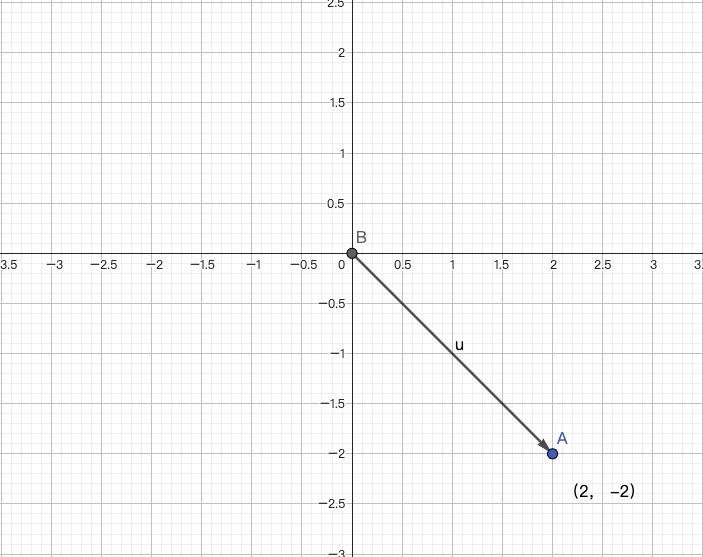
\includegraphics[width=0.5\textwidth]{asset/20230825222021.png}
  \caption{}
  \label{fig:img4_1}
\end{figure}

这个向量在平面直角坐标性里面可以用一个箭头来表示, 然后拿矩阵和向量做一个乘法运算会得到什么结果呢?让我们先来计算一下:

\begin{align*}
  \begin{split}
    & \begin{bmatrix} cos90^\circ & -sin90^\circ \\ sin90^\circ & cos90^\circ \end{bmatrix}
    \begin{bmatrix} 2 \\ -2 \end{bmatrix} 
    = \begin{bmatrix} 2cos90^\circ + 2sin90^\circ \\ 2sin90^\circ - 2cos90^\circ \end{bmatrix} 
    = \begin{bmatrix} 2 \\ 2 \end{bmatrix}
  \end{split}
\end{align*}

再把得到的这个向量也放到坐标系里去(图: \ref{fig:img4_2}):

\begin{figure}[ht]
  \centering
  \caption{}
  \label{fig:img4_2}
  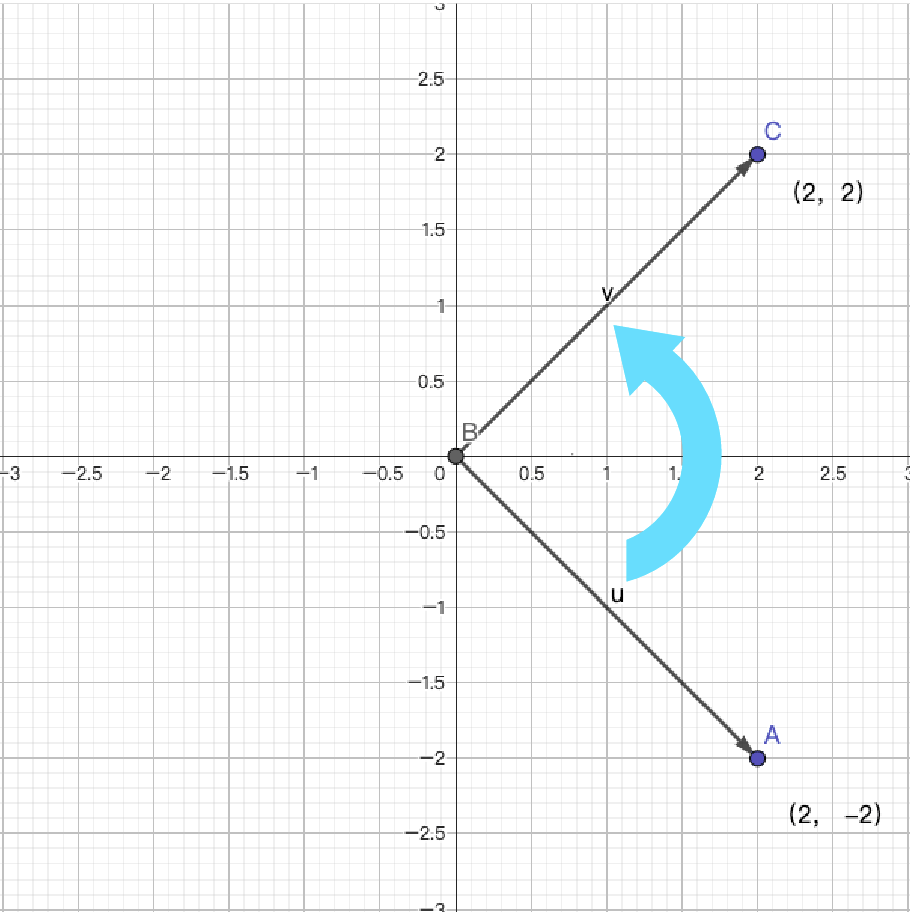
\includegraphics[width=0.5\textwidth]{asset/20230825225602.png}
\end{figure}

我们发现从几何意义上面来说相当于逆时针旋转了 90 度. 所以矩阵在几何上面对应的意义是这个例子里面的旋转变换. 把一个向量旋转一下, 然后这个 90 度就是这个矩称里面的三角函数值的度数. 

除了旋转之外, 还有一个是可以拉伸, 拉伸在之后的课程里面会碰到, 这里给大家举一个旋转的例子, 带大家感受一下矩阵的几何意义. 

\section{矩阵的转置}

矩阵的转置就是沿对角线为对称轴, 把矩阵翻转一下. 或者说这个矩阵行列进行互换. 我们在 Python 课程中后面两节有讲到数据的行转列, 忘记的小伙伴可以再回去复习一下. 

也就是说,本来$1 \quad 2 \quad 3 \quad 4$是第一行, 转置了之后就变成了第一列. $5 \quad 6 \quad 7 \quad 8$是第二行转置了之后第二列, 后面的第三行变成第三列, 这个叫做转置:

\begin{align*}
  \begin{bmatrix} 1 & 2 & 3 & 4 \\ 5 & 6 & 7 & 8 \\ 9 & a & b & c \end{bmatrix}^T
  \Rightarrow \begin{bmatrix} 1 & 5 & 9 \\ 2 & 6 & a \\ 3 & 7 & b \\ 4 & 8 & c \end{bmatrix}
\end{align*}

这个部分还是很好理解. 

\section{矩阵的逆}

矩阵的逆有点像数里面的除法, 就是矩阵乘上它相对应的逆之后, 得到了一个单位矩阵, 这个单位矩阵它是只有在斜对角上是 1, 其他地方的元素全部都是 0 的一个状态. 

\begin{align*}
  \begin{split}
    A^{-1}\mbox{满足}:AA^{-1}=I, \mbox{其中 I 为}
    \begin{bmatrix} 1 & \cdots & 0 \\ \vdots & \ddots &\vdots \\ 0 & \cdots & 1 \end{bmatrix}
  \end{split}
\end{align*}

求解方程组, 就是通过求矩阵系数的逆去做的. 当然逆的作用在高等代数里面非常多, 就不一一缀述了. 大家先知道是怎么一回事, 后面还会专门去讲. 

这里再给大家说一个题外话, AI 这个行业虽然现在世界上中国和美国是并驾齐驱的两个大国. 就是在 AI 领域基本上前沿的研究主要都是中美两国的研究人员做出的. 但是在这个领域里面的文献资料什么的还是以英文为主, 所以我也建议大家多关注一下或者多提升一下自己的英语能力. 你不能拿到一篇 AI 的论文, 想了解它这里面的算法原理以及它是怎么实现的, 可还看不懂 \footnote{之后我会专门写一篇如何去读论文的文章,放在「BI」部分写吧,大家可以关注我后续课程。}. 

而且我有自己的一些感受可以跟大家分享一下, 越是这种专业性比较强的领域, 其实英语上手的难度就越不大. 首先不可能像 GRE 阅读题那样考到怀疑人生, 看完 GRE 阅读再回头看托福的阅读题, 就像是大学教材和初中教材一样那种感觉. 所以某一个领域的东西它的语法结构不会很复杂. 只需要掌握那个领域特殊的一些术语就行了. 剩下的语法规则我觉得高中英语就够了. 

这个不应该成为大家一个障碍, 所以推荐大家从现在开始就去提升一下自己的英文方面的阅读能力. 从阅读开始再慢慢的扩展到其他领域. 